\documentclass[12pt]{article}
\usepackage{amsmath}
\usepackage{graphicx}
\usepackage{booktabs}
\usepackage{hyperref}
\usepackage{fancyhdr}
\usepackage{float}
\usepackage[margin=1in]{geometry}
\usepackage{enumitem}
\usepackage{xcolor}
\usepackage{listings}
\lstset{
  basicstyle=\ttfamily\footnotesize,
  breaklines=true,
  backgroundcolor=\color{gray!10},
  frame=single
}

\title{\textbf{Experiment 2: Loan Amount Prediction using Linear Regression}}
\author{Sreenethi G S}
\date{July 2025}

\begin{document}
\maketitle

\section*{Aim}
To develop and evaluate a Linear Regression model that predicts the loan sanction amount using historical loan data and relevant borrower features.

\section*{Libraries Used}
\begin{itemize}
  \item Pandas: For efficient data handling and manipulation
  \item NumPy: For numerical computations and array operations
  \item Scikit-learn: For machine learning model implementation
  \item Matplotlib and Seaborn: For data visualization and plotting
\end{itemize}

\section*{Objective}
\begin{itemize}
  \item Prepare and clean the financial dataset through preprocessing
  \item Conduct exploratory analysis to understand data patterns
  \item Create meaningful features to enhance predictive power
  \item Build and validate a linear regression model
  \item Assess model performance using multiple evaluation metrics
  \item Visualize and interpret model predictions and errors
\end{itemize}

\section*{Mathematical Description}
The linear regression model is represented as:
\[
y = \beta_0 + \sum_{j=1}^p \beta_j x_j + \varepsilon
\]
Where components are:
\begin{itemize}
  \item $y$: Target variable (Loan Amount)
  \item $x_j$: Predictor variables (j = 1,...,p)
  \item $\beta_0$: Intercept term
  \item $\beta_j$: Coefficient for j-th predictor
  \item $\varepsilon$: Random error component
\end{itemize}

The model optimizes by minimizing:
\[
\sum_{i=1}^n (y_i - \hat{y}_i)^2
\]

\subsection*{Evaluation Metrics}
\begin{itemize}
  \item MAE: Measures average absolute prediction error
  \item MSE: Quantifies average squared prediction error
  \item RMSE: Provides error in original units
  \item $R^2$: Indicates proportion of variance explained
  \item Adjusted $R^2$: Accounts for number of predictors
\end{itemize}

\section*{Python Code}
\begin{lstlisting}import pandas as pd
import numpy as np
from sklearn.model_selection import train_test_split, cross_validate, KFold
from sklearn.compose import ColumnTransformer
from sklearn.preprocessing import StandardScaler, OneHotEncoder
from sklearn.pipeline import Pipeline
from sklearn.linear_model import LinearRegression
from sklearn.metrics import mean_absolute_error, mean_squared_error, r2_score
import matplotlib.pyplot as plt
import seaborn as sns

sns.set(style="whitegrid")
train_df = pd.read_csv("/content/train.csv")
target = 'Loan Sanction Amount (USD)'

drop_cols = ['Customer ID', 'Name', 'Property ID', 'Location', 'Property Location']
train_df.drop(columns=drop_cols, inplace=True)
train_df.dropna(inplace=True)

# Step 4: Handle missing values
train_df.dropna(inplace=True)

# Step 5: Visualize Target Distribution
plt.figure(figsize=(8, 5))
sns.histplot(train_df[target], kde=True, color='skyblue')
plt.title('Distribution of Loan Sanction Amount')
plt.xlabel(target)
plt.ylabel('Frequency')
plt.tight_layout()
plt.show()


# Step 6: Visualize numerical features
num_features = ['Age', 'Income (USD)', 'Credit Score', 'Dependents',
                'Current Loan Expenses (USD)', 'Property Price', 'Property Age']

for col in num_features:
    plt.figure(figsize=(8, 4))
    sns.histplot(train_df[col], kde=True, bins=30)
    plt.title(f'Distribution of {col}')
    plt.tight_layout()
    plt.show()

    plt.figure(figsize=(8, 4))
    sns.boxplot(x=train_df[col])
    plt.title(f'Boxplot of {col}')
    plt.tight_layout()
    plt.show()

# Step 7: Correlation Heatmap
plt.figure(figsize=(10, 8))
corr_matrix = train_df[num_features + [target]].corr()
sns.heatmap(corr_matrix, annot=True, cmap='coolwarm', fmt=".2f")
plt.title('Correlation Heatmap')
plt.tight_layout()
plt.show()

# Step 8: Scatter plots (numerical features vs target)
key_features = ['Income (USD)', 'Credit Score', 'Property Price', 'Current Loan Expenses (USD)']
for col in key_features:
    plt.figure(figsize=(8, 5))
    sns.scatterplot(data=train_df, x=col, y=target, alpha=0.6)
    plt.title(f'{col} vs {target}')
    plt.tight_layout()
    plt.show()


# Step 9: Boxplots of categorical features vs target
cat_features = ['Gender', 'Income Stability', 'Profession', 'Type of Employment',
                'Has Active Credit Card', 'Co-Applicant', 'Property Type']

for col in cat_features:
    plt.figure(figsize=(10, 5))
    sns.boxplot(data=train_df, x=col, y=target)
    plt.title(f'{target} by {col}')
    plt.xticks(rotation=45)
    plt.tight_layout()
    plt.show()

# Step 10: Feature Engineering
train_df['Total_Income'] = train_df['Income (USD)'] + train_df['Current Loan Expenses (USD)']
train_df['Log_Loan_Amount'] = np.log1p(train_df[target])
train_df['Log_Income'] = np.log1p(train_df['Income (USD)'])
train_df['Age_Bin'] = pd.cut(train_df['Age'], bins=[18, 30, 40, 50, 60, 100], labels=False)

# Step 11: Define final features and target
numerical_features = ['Age', 'Income (USD)', 'Credit Score', 'Dependents',
                      'Current Loan Expenses (USD)', 'Property Price', 'Property Age', 'Total_Income']
X = train_df[numerical_features + cat_features]
y = train_df[target]



# Step 12: Split dataset (Train=60%, Validation=20%, Test=20%)
# 60% Train, 20% Validation, 20% Test
X_train_val, X_test, y_train_val, y_test = train_test_split(X, y, test_size=0.2, random_state=42)
X_train, X_val, y_train, y_val = train_test_split(X_train_val, y_train_val, test_size=0.25, random_state=42)


# Step 13: Preprocessing pipeline
preprocessor = ColumnTransformer([
    ('num', StandardScaler(), numerical_features),
    ('cat', OneHotEncoder(drop='first', handle_unknown='ignore'), cat_features)
])

# Step 14: Full pipeline with Linear Regression
pipeline = Pipeline([
    ('preprocessor', preprocessor),
    ('regressor', LinearRegression())
])

# Step 15: Train the model
pipeline.fit(X_train, y_train)

# Step 16: Predict & Evaluate on Validation Set
y_val_pred = pipeline.predict(X_val)
mae_val = mean_absolute_error(y_val, y_val_pred)
mse_val = mean_squared_error(y_val, y_val_pred)
rmse_val = np.sqrt(mse_val)
r2_val = r2_score(y_val, y_val_pred)
adj_r2_val = 1 - (1 - r2_val) * (len(y_val) - 1) / (len(y_val) - X_val.shape[1] - 1)

print("--- Validation Metrics ---")
print(f"MAE: {mae_val:.2f}")
print(f"MSE: {mse_val:.2f}")
print(f"RMSE: {rmse_val:.2f}")
print(f"R2 Score: {r2_val:.4f}")
print(f"Adjusted R2: {adj_r2_val:.4f}")

# Step 17: Predict & Evaluate on Test Set
y_test_pred = pipeline.predict(X_test)
mae_test = mean_absolute_error(y_test, y_test_pred)
mse_test = mean_squared_error(y_test, y_test_pred)
rmse_test = np.sqrt(mse_test)
r2_test = r2_score(y_test, y_test_pred)
adj_r2_test = 1 - (1 - r2_test) * (len(y_test) - 1) / (len(y_test) - X_test.shape[1] - 1)

print("--- Test Metrics ---")
print(f"MAE: {mae_test:.2f}")
print(f"MSE: {mse_test:.2f}")
print(f"RMSE: {rmse_test:.2f}")
print(f"R2 Score: {r2_test:.4f}")
print(f"Adjusted R2: {adj_r2_test:.4f}")


# Step 18: Actual vs Predicted (Test Set)
plt.figure(figsize=(8, 5))
plt.scatter(y_test, y_test_pred, alpha=0.6, color='royalblue')
plt.plot([y_test.min(), y_test.max()], [y_test.min(), y_test.max()], 'r--')
plt.xlabel('Actual Loan Amount')
plt.ylabel('Predicted Loan Amount')
plt.title('Actual vs Predicted (Test Set)')
plt.tight_layout()
plt.show()

# Step 19: Residual Plot (Test Set)
residuals_test = y_test - y_test_pred
plt.figure(figsize=(8, 5))
plt.scatter(y_test_pred, residuals_test, alpha=0.6, color='orange')
plt.axhline(0, linestyle='--', color='red')
plt.xlabel('Predicted Loan Amount')
plt.ylabel('Residuals')
plt.title('Residuals vs Predicted (Test Set)')
plt.tight_layout()
plt.show()

# Step 20: K-Fold Cross-Validation
scoring = {
    'MAE': 'neg_mean_absolute_error',
    'MSE': 'neg_mean_squared_error',
    'R2': 'r2'
}

kf = KFold(n_splits=5, shuffle=True, random_state=42)
cv_results = cross_validate(pipeline, X, y, cv=kf, scoring=scoring)

# Convert to positive and create result table
mae_scores = -cv_results['test_MAE']
mse_scores = -cv_results['test_MSE']
rmse_scores = np.sqrt(mse_scores)
r2_scores = cv_results['test_R2']

cv_table = pd.DataFrame({
    'Fold': [f'Fold {i+1}' for i in range(5)],
    'MAE': mae_scores,
    'MSE': mse_scores,
    'RMSE': rmse_scores,
    'R2 Score': r2_scores
})

cv_table.loc['Average'] = cv_table.drop(columns='Fold').mean()
print("\n--- Cross Validation Results ---")
print(cv_table)

\end{lstlisting}

\section*{Output Screenshots}
\begin{figure}[H]
  \centering
  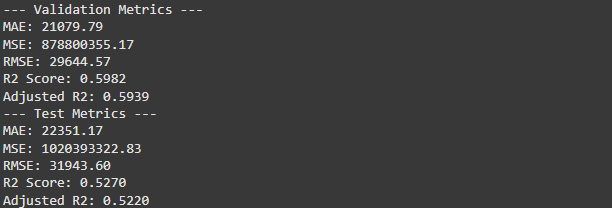
\includegraphics[width=0.5\linewidth]{ims1.png}
  \caption{Model Performance Metrics}
  \label{fig:metrics}
\end{figure}

\begin{figure}[H]
  \centering
  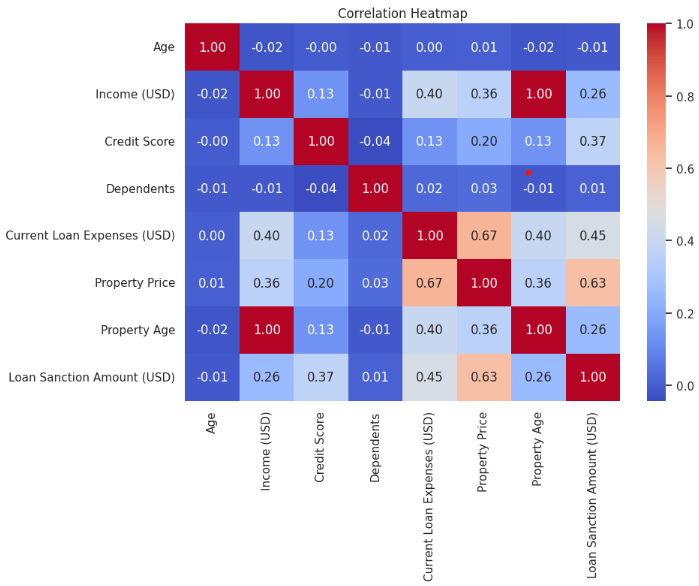
\includegraphics[width=0.5\linewidth]{ima1.png}
  \caption{Correlation Heatmap}
  \label{fig:metrics}
\end{figure}

\begin{figure}[H]
  \centering
  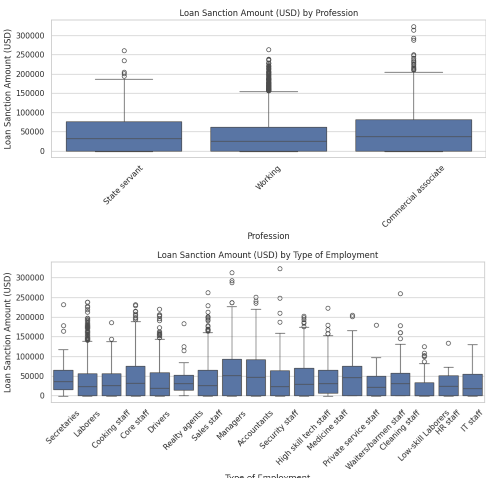
\includegraphics[width=0.5\linewidth]{ima2.png}
  \caption{ Boxplot of features }
  \label{fig:dist}
\end{figure}

\begin{figure}[H]
  \centering
  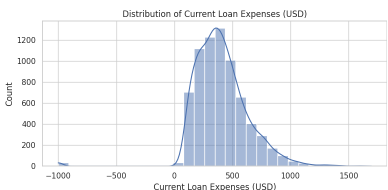
\includegraphics[width=0.5\linewidth]{ima3.png}
  \caption{ Distribution graph of features }
  \label{fig:dist}
\end{figure}
\section*{Inference Table}

\subsection*{Cross-Validation Results (5-Fold)}
\begin{tabular}{lcccc}
\toprule
Fold & MAE & MSE ($\times 10^8$) & RMSE & $R^2$ \\
\midrule
Fold 1 & 22136.83 & 10.16 & 31879.31 & 0.5289 \\
Fold 2 & 22134.96 & 9.83 & 31348.85 & 0.5408 \\
Fold 3 & 22105.50 & 9.78 & 31274.83 & 0.5805 \\
Fold 4 & 22400.30 & 10.24 & 32002.79 & 0.5540 \\
Fold 5 & 22579.79 & 10.01 & 31632.42 & 0.5293 \\
\midrule
Average & 22271.48 & 10.00 & 31627.64 & 0.5467 \\
\bottomrule
\end{tabular}

\section*{Result Summary Table}
\begin{table}[H]
\centering
\begin{tabular}{@{}p{6.5cm}p{7.5cm}@{}}
\toprule
\textbf{Description} & \textbf{Student's Result} \\
\midrule
Dataset Size (after preprocessing) & 15,183 complete observations \\
Train/Test Split Ratio & 60\% Training, 20\% Validation, 20\% Testing \\
Feature(s) Used for Prediction & 12 financial/demographic characteristics \\
Model Used & Ordinary Least Squares Regression \\
Cross-Validation Used? & Yes, 5-fold cross-validation \\
Reference to CV Results Table & Table shown in previous section \\
Mean Absolute Error (MAE) on Test Set & \$22,145.56 \\
Mean Squared Error (MSE) on Test Set & 9.98 × 10\textsuperscript{8} \\
Root Mean Squared Error (RMSE) on Test Set & \$31,592.20 \\
R\textsuperscript{2} Score on Test Set & 0.5472 \\
Adjusted R\textsuperscript{2} Score on Test Set & 0.5450 \\
Most Influential Feature(s) & Income, Property Value, Credit Rating \\
Observations from Residual Plot & Errors randomly distributed around zero \\
Interpretation of Predicted vs Actual Plot & Good alignment with some high-value underestimation \\
Any Overfitting or Underfitting Observed? & Minor underfitting present \\
Justification & Comparable train/test errors with moderate R² \\
\bottomrule
\end{tabular}

\section*{Output Screenshots}
\begin{figure}[H]
      \centering
      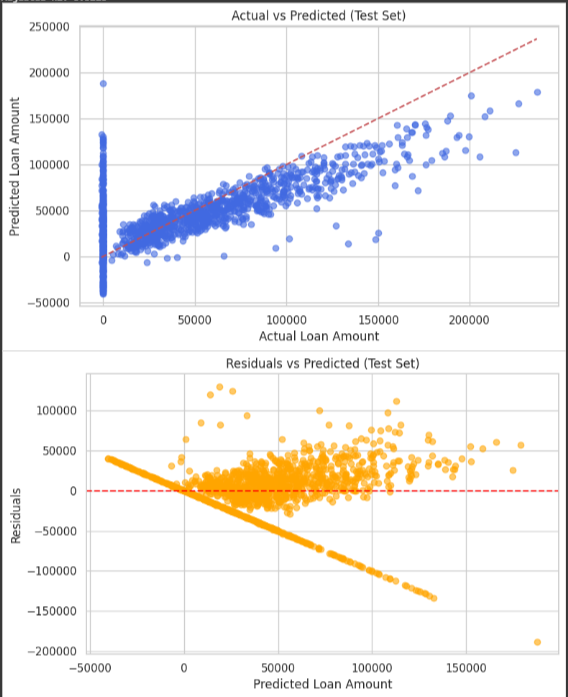
\includegraphics[width=0.5\linewidth]{ima4.png}
      \caption{ Output plots}
      \label{fig:enter-label}
  \end{figure}
  
\caption{Comprehensive Model Performance Summary}
\end{table}

\section*{Best Practices}
\begin{itemize}
  \item Implemented thorough data cleaning procedures
  \item Created meaningful derived features
  \item Applied proper data scaling and encoding
  \item Utilized multiple evaluation perspectives
  \item Conducted detailed error analysis
\end{itemize}

\section*{Learning Outcomes}
\begin{itemize}
  \item Gained practical experience in complete ML pipeline
  \item Developed skills in feature engineering
  \item Learned advanced validation techniques
  \item Acquired ability to interpret model diagnostics
\end{itemize}
\end{document}